\documentclass{article}
\usepackage[utf8]{inputenc}

\usepackage[paperwidth=8.5in, paperheight=11in, top=1in, bottom=.5in, left=.5in, right=.5in]{geometry}
\usepackage{fancyhdr, graphicx,tikz,amsmath,multicol,paracol}
\usepackage[inline]{enumitem}


\pagestyle{fancy}
\lhead{\large{\textbf{Module 3: Linear Functions (LF) - Readiness Assurance Test}}}
\chead{}
\rhead{}
\lfoot{}
\cfoot{}
%\rfoot{\thepage/\pageref{LastPage} }
\setlength{\headheight}{14pt} %added in bc warning

%%% LIST ANSWER KEY HERE

% 1 C
% 2 A
% 3 D
% 4 B
% 5 B
% 6 C
% 7 D
% 8 C
% 9 B
% 10 B

\begin{document}


\begin{enumerate}


% Point plots on the coordinate plane.

\item How can you write points $A$ and $B$ as ordered pairs?
\begin{center}
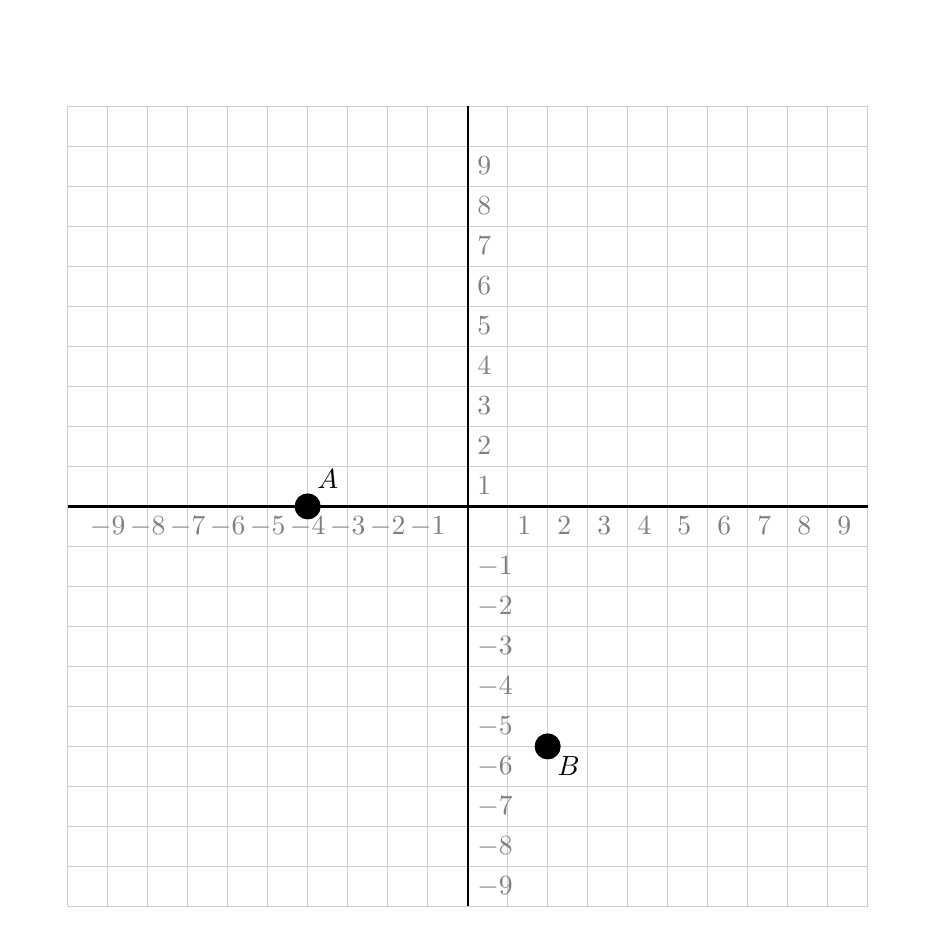
\begin{tikzpicture}[x=0.2in,y=0.2in]
\fill[white] (-11,-11) rectangle (11,11);
\draw[black!20,step=1] (-10,-10) grid (10,10);
\draw[thick] (0,-10) -- (0,10);
\draw[thick] (-10,0) -- (10,0);
\node[circle,fill] at (-4,0) {};
\node[anchor=south west] at (-4,0.2) {$A$};
\node[circle,fill] at (2,-6) {};
\node[anchor=north west] at (2,-6) {$B$};
\foreach \i in {-9,...,-1}
  {\node[anchor=north,thin,gray] at (\i,0) {$\i$};
  \node[anchor=north west,thin,gray] at (0,\i) {$\i$};}
\foreach \i in {1,...,9}
  {\node[anchor=north west,thin,gray] at (\i,0) {$\i$};
  \node[anchor=north west,thin,gray] at (0,\i) {$\i$};}
\end{tikzpicture}
\end{center}

  \begin{enumerate}
  
  \item $A(-4,0)$ and $B(-2,-6)$  
  \item $A(4,0)$ and $B(2,-6)$
  \item $A(-4,0)$ and $B(2,-6)$ %correct 
  \item $A(0,-4)$ and $B(-2,-6)$
  
  \end{enumerate}

% Find and plot x- and y-intercepts.

\item Suppose a graph has an $x$-intercept of $-1$ and a $y$-intercept of $-5$. How can we write these intercepts as ordered pairs?

  \begin{enumerate}
  \item $x$-intercept: $(-1,0)$; $y$-intercept: $(0,-5)$ %correct 
  \item $x$-intercept: $(0,-1)$; $y$-intercept: $(-5,0)$
  \item $x$-intercept: $(-1,0)$; $y$-intercept: $(-5,0)$
  \item $x$-intercept: $(0,-1)$; $y$-intercept: $(0,-5)$
  \end{enumerate}

% Evaluate a function at a given value.

\item What is the value of the expression $5(x-2y)+(2-x)^2$ when $x=3$ and $y=-2$?

  \begin{enumerate}
  \begin{multicols}{4}
  \item $20$
  \item $50$
  \item $1156$
  \item $36$ %correct
   \end{multicols}
  \end{enumerate}
  
 \item Find $f(4)$ given $f(x)=5x^2-5x+7$.

  \begin{enumerate}
  \begin{multicols}{4}
  \item $57$  
  \item $67$ %correct 
  \item $3$
  \item $107$
  \end{multicols}
  \end{enumerate}

 \item Given that $g(x)=3x-5$, which of the following statements is true?

  \begin{enumerate}
  \begin{multicols}{4}
  \item $g(0)=0$  
  \item $g(3)=4$ %correct 
  \item $g(4)=3$
  \item $g(5)=0$
  \end{multicols}
  \end{enumerate}
  
\pagebreak

% Solve a linear equation for a variable.

\item Which of the following would be the best choice for the first step in solving for $b$ in the equation: $-8+2b=20$?

  \begin{enumerate}
  \item subtract $8$ from both sides of the equation
  \item multiply both sides of the equation by $2$
  \item add $8$ to both sides of the equation %correct
  \item divide both sides of the equation by $-2$
  \end{enumerate}
  
  \item Given the equation, $5x-6y=5$, solve for $y$ in terms of $x$.

  \begin{enumerate}
  \begin{multicols}{4}
  \item $y=5-5x$
  \item $y=5-\dfrac{5x}{6}$
  \item $y=-5x-\dfrac{5}{6}$
  \item $y=\dfrac{5}{6}x-\dfrac{5}{6}$ %correct
   \end{multicols}
  \end{enumerate}

\item Solve the equation: $3(x+6)=30$.

  \begin{enumerate}
  \begin{multicols}{4}
  \item $5$
  \item $8$
  \item $4$ %correct
  \item $14$ 
   \end{multicols}
  \end{enumerate}

\item Solve for $x$: $\dfrac{3}{5}(x+2)=x-4$.

  \begin{enumerate}
  \begin{multicols}{4}
  \item $8$
  \item $13$ %correct
  \item $15$ 
  \item $23$ 
   \end{multicols}
  \end{enumerate}

% Define and find reciprocals.

\item What is the reciprocal of $\dfrac{2}{3}$?

  \begin{enumerate}
  \begin{multicols}{4}
  \item $-\dfrac{2}{3}$
  \item $\dfrac{3}{2}$ %correct
  \item $-\dfrac{3}{2}$
  \item $\dfrac{2}{3}$ 
   \end{multicols}
  \end{enumerate}

\end{enumerate}


\end{document}